\documentclass[11pt,]{article}

\usepackage{lmodern}

\usepackage{amssymb,amsmath}
\usepackage{ifxetex,ifluatex}
\usepackage{fixltx2e} % provides \textsubscript
\ifnum 0\ifxetex 1\fi\ifluatex 1\fi=0 % if pdftex
  \usepackage[T1]{fontenc}
  \usepackage[utf8]{inputenc}
\else % if luatex or xelatex
  \ifxetex
    \usepackage{mathspec}
    \usepackage{xltxtra, xunicode}
  \else
    \usepackage{fontspec}
  \fi
  \defaultfontfeatures{Mapping=tex-text, Scale=MatchLowercase}
  \newcommand{\euro}{€}
\fi

% use upquote if available, for straight quotes in verbatim environments
\IfFileExists{upquote.sty}{\usepackage{upquote}}{}
% use microtype if available
\IfFileExists{microtype.sty}{%
\usepackage{microtype}
\UseMicrotypeSet[protrusion]{basicmath} % disable protrusion for tt fonts
}{}
\usepackage[top=0.5in, bottom=.4in, left = 1in, right=1in, includeheadfoot]{geometry}
\ifxetex
  \usepackage[setpagesize=false, % page size defined by xetex
              unicode=false, % unicode breaks when used with xetex
              xetex]{hyperref}
\else
  \usepackage[unicode=true]{hyperref}
\fi
\hypersetup{breaklinks=true,
            bookmarks=true,
            pdfauthor={Martin Frigaard},
            pdftitle={The Grammar of Graphics},
            colorlinks=true,
            citecolor=blue,
            urlcolor=blue,
            linkcolor=magenta,
            pdfborder={0 0 0}}
\urlstyle{same}  % don't use monospace font for urls
\usepackage{color}
\usepackage{fancyvrb}
\newcommand{\VerbBar}{|}
\newcommand{\VERB}{\Verb[commandchars=\\\{\}]}
\DefineVerbatimEnvironment{Highlighting}{Verbatim}{commandchars=\\\{\}}
% Add ',fontsize=\small' for more characters per line
\usepackage{framed}
\definecolor{shadecolor}{RGB}{248,248,248}
\newenvironment{Shaded}{\begin{snugshade}}{\end{snugshade}}
\newcommand{\AlertTok}[1]{\textcolor[rgb]{0.94,0.16,0.16}{#1}}
\newcommand{\AnnotationTok}[1]{\textcolor[rgb]{0.56,0.35,0.01}{\textbf{\textit{#1}}}}
\newcommand{\AttributeTok}[1]{\textcolor[rgb]{0.77,0.63,0.00}{#1}}
\newcommand{\BaseNTok}[1]{\textcolor[rgb]{0.00,0.00,0.81}{#1}}
\newcommand{\BuiltInTok}[1]{#1}
\newcommand{\CharTok}[1]{\textcolor[rgb]{0.31,0.60,0.02}{#1}}
\newcommand{\CommentTok}[1]{\textcolor[rgb]{0.56,0.35,0.01}{\textit{#1}}}
\newcommand{\CommentVarTok}[1]{\textcolor[rgb]{0.56,0.35,0.01}{\textbf{\textit{#1}}}}
\newcommand{\ConstantTok}[1]{\textcolor[rgb]{0.00,0.00,0.00}{#1}}
\newcommand{\ControlFlowTok}[1]{\textcolor[rgb]{0.13,0.29,0.53}{\textbf{#1}}}
\newcommand{\DataTypeTok}[1]{\textcolor[rgb]{0.13,0.29,0.53}{#1}}
\newcommand{\DecValTok}[1]{\textcolor[rgb]{0.00,0.00,0.81}{#1}}
\newcommand{\DocumentationTok}[1]{\textcolor[rgb]{0.56,0.35,0.01}{\textbf{\textit{#1}}}}
\newcommand{\ErrorTok}[1]{\textcolor[rgb]{0.64,0.00,0.00}{\textbf{#1}}}
\newcommand{\ExtensionTok}[1]{#1}
\newcommand{\FloatTok}[1]{\textcolor[rgb]{0.00,0.00,0.81}{#1}}
\newcommand{\FunctionTok}[1]{\textcolor[rgb]{0.00,0.00,0.00}{#1}}
\newcommand{\ImportTok}[1]{#1}
\newcommand{\InformationTok}[1]{\textcolor[rgb]{0.56,0.35,0.01}{\textbf{\textit{#1}}}}
\newcommand{\KeywordTok}[1]{\textcolor[rgb]{0.13,0.29,0.53}{\textbf{#1}}}
\newcommand{\NormalTok}[1]{#1}
\newcommand{\OperatorTok}[1]{\textcolor[rgb]{0.81,0.36,0.00}{\textbf{#1}}}
\newcommand{\OtherTok}[1]{\textcolor[rgb]{0.56,0.35,0.01}{#1}}
\newcommand{\PreprocessorTok}[1]{\textcolor[rgb]{0.56,0.35,0.01}{\textit{#1}}}
\newcommand{\RegionMarkerTok}[1]{#1}
\newcommand{\SpecialCharTok}[1]{\textcolor[rgb]{0.00,0.00,0.00}{#1}}
\newcommand{\SpecialStringTok}[1]{\textcolor[rgb]{0.31,0.60,0.02}{#1}}
\newcommand{\StringTok}[1]{\textcolor[rgb]{0.31,0.60,0.02}{#1}}
\newcommand{\VariableTok}[1]{\textcolor[rgb]{0.00,0.00,0.00}{#1}}
\newcommand{\VerbatimStringTok}[1]{\textcolor[rgb]{0.31,0.60,0.02}{#1}}
\newcommand{\WarningTok}[1]{\textcolor[rgb]{0.56,0.35,0.01}{\textbf{\textit{#1}}}}
\usepackage{longtable,booktabs}
\usepackage{graphicx}
\makeatletter
\def\maxwidth{\ifdim\Gin@nat@width>\linewidth\linewidth\else\Gin@nat@width\fi}
\def\maxheight{\ifdim\Gin@nat@height>\textheight\textheight\else\Gin@nat@height\fi}
\makeatother
% Scale images if necessary, so that they will not overflow the page
% margins by default, and it is still possible to overwrite the defaults
% using explicit options in \includegraphics[width, height, ...]{}
\setkeys{Gin}{width=\maxwidth,height=\maxheight,keepaspectratio}
% \setlength{\parindent}{0pt}
\setlength{\parskip}{6pt plus 2pt minus 1pt}
\setlength{\emergencystretch}{3em}  % prevent overfull lines
\setcounter{secnumdepth}{5}

%%% Use protect on footnotes to avoid problems with footnotes in titles
\let\rmarkdownfootnote\footnote%
\def\footnote{\protect\rmarkdownfootnote}

%%% Change title format to be more compact
\usepackage{titling}

% % Create subtitle command for use in maketitle
% \newcommand{\subtitle}[1]{
%   \posttitle{\large}
% }

% \setlength{\droptitle}{-2em}
  \title{The Grammar of Graphics}
  % \pretitle{\vspace{\droptitle}\centering\huge}
  \author{Martin Frigaard}
  % \preauthor{\centering\large\emph}
  % \postauthor{\par}
  % \predate{\centering\large\emph}
  % \postdate{\par}
  \date{2021-05-01}

%% --------- above is almost identical with default rmarkdown
%% document formatting
 % colors for tables and text
\usepackage{ragged2e} % justifying text
\usepackage{setspace} % spacing commands, automatically makes captions single-spaced
  \setstretch{1.2} \frenchspacing
\usepackage{lastpage} % access number of last page for numbering in margin

%% fonts setup
\usepackage{gensymb} %degree symbol
\usepackage{array}
\usepackage{multirow}
\usepackage{xcolor}
\usepackage{wrapfig}
\usepackage{float}
\usepackage{colortbl}
\usepackage{pdflscape}
\usepackage{tabu}
\usepackage{threeparttable}
\usepackage{threeparttablex}
\usepackage{makecell}
\usepackage[hang]{footmisc}

%% tables and figures

% include section number in figure and table numbers, renew in each section
\usepackage{chngcntr}
\counterwithin{table}{section}
\counterwithin{figure}{section}

\robustify\tnote

% table/figure captions (titles and legends)

% \usepackage{caption}
% % \DeclareCaptionFormat{llap}{\llap{#1#2}#3\par} % table / figure number in left margin
% \DeclareCaptionLabelSeparator{spc}{\hspace{.075 in}} % space between table number and caption
% \captionsetup{font={color=blue, sf}, singlelinecheck=off, margin= 15pt, skip=4pt, size=small, labelfont={sc, sf}, format=llap, labelsep=spc,singlelinecheck=no} % same font as headers
% 
% table/figure captions (titles and legends)
\usepackage[singlelinecheck=false]{caption} % left justify table captions
\captionsetup{font={color=black, sf}, skip=4pt, size=small, labelfont=sf, labelsep = period} % color and spacing between caption and table proper, updated 

\makeatletter
\let\runtitle\@title
\makeatother

\usepackage{fancyhdr}
\pagestyle{fancy}
\fancyhf{}
\renewcommand{\headrulewidth}{0pt}
\rhead{\footnotesize \nouppercase{\sc short title} \hspace{.025 in} \hspace{.055 in} \thepage \hspace{.01 in} / \pageref*{LastPage}}

   
      \renewcommand{\footrulewidth}{0.5pt}
   \cfoot{\footnotesize
   Martin J Frigaard \hspace{.025 in} $\cdot$ \hspace{.05 in} Senior Clinical Programmer, BioMarin \hspace{.025 in} $\cdot$ \hspace{.05 in} 1+503.333.0531 \hspace{.025 in} $\cdot$ \hspace{.05 in} mjfrigaard@pm.me
   }
   
\fancypagestyle{firststyle}
{
   \fancyhf{}
      \renewcommand{\footrulewidth}{0.5pt}
   \cfoot{\footnotesize
   Martin J Frigaard \hspace{.025 in} $\cdot$ \hspace{.05 in} Senior Clinical Programmer, BioMarin \hspace{.025 in} $\cdot$ \hspace{.05 in} 1+503.333.0531 \hspace{.025 in} $\cdot$ \hspace{.05 in} mjfrigaard@pm.me
   }
   }

\fancypagestyle{nofooter}
{
   \fancyfoot{}
   \renewcommand{\footrulewidth}{0.0pt}
}

\setlength\parindent{0pt}

\usepackage{titlesec}
\titleformat*{\section}{\sc \large \color[rgb]{0,0,0}}
\titleformat*{\subsection}{\large}
\titleformat*{\subsubsection}{\normalsize}
\titlespacing\section{0pt}{8pt plus 2pt minus 2pt}{0pt plus 2pt minus 2pt}
\titlespacing\subsection{0pt}{6pt plus 2pt minus 2pt}{-2pt plus 2pt minus 2pt}
\titlespacing\subsubsection{0pt}{2pt plus 2pt minus 2pt}{-3pt plus 2pt minus 2pt}


% set up title page
\pretitle{
\begin{flushleft}\LARGE
}

\posttitle{
  \end{flushleft}
}

\preauthor{\par\begin{flushleft}\large\vskip -.5em}
\postauthor{\end{flushleft}}

\predate{\par\begin{flushleft}\large\vskip -1em}
\postdate{\end{flushleft}  }

\makeatletter
\def\@seccntformat#1{\llap{\csname the#1\endcsname \hspace{.075 in}}}
\makeatother

% suppress chapter in section numbering
\renewcommand*\thesection{\arabic{section}}

% spacing of bulleted lists
\usepackage{enumitem} %control spacing of enumerated items
\setlist[itemize]{noitemsep, topsep=0pt}

%% remove 'abstract' title, justify text
\renewcommand{\abstractname}{\large}
\renewenvironment{abstract} {\abstractname \justifying \rm \normalsize }

\newlength\tbspace
\setlength\tbspace{.25in}

% units.
%\usepackage{units}

%% change fontsize of R code
\let\oldShaded\Shaded
\let\endoldShaded\endShaded
\renewenvironment{Shaded}{\footnotesize\oldShaded}{\endoldShaded}

%% change fontsize of output
\let\oldverbatim\verbatim
\let\endoldverbatim\endverbatim
\renewenvironment{verbatim}{\footnotesize\oldverbatim}{\endoldverbatim}

\def\tightlist{}



% Redefines (sub)paragraphs to behave more like sections
\ifx\paragraph\undefined\else
\let\oldparagraph\paragraph
\renewcommand{\paragraph}[1]{\oldparagraph{#1}\mbox{}}
\fi
\ifx\subparagraph\undefined\else
\let\oldsubparagraph\subparagraph
\renewcommand{\subparagraph}[1]{\oldsubparagraph{#1}\mbox{}}
\fi


\begin{document}
\maketitle

\thispagestyle{firststyle}


{
\hypersetup{linkcolor=black}
\setcounter{tocdepth}{2}
\tableofcontents
}

The \texttt{ggplot2} package is one of most commonly used tools for data
visualizations. For more on the grammar, see the online text titled,
\href{https://ggplot2-book.org/}{ggplot2: Elegant Graphics for Data
Analysis}. If you're looking for a cookbook (graphs and code to build
them), see the \href{https://r-graphics.org/}{R Graphics Cookbook, 2nd
edition}.

\hypertarget{why-have-a-grammar-of-graphics}{%
\subsection{Why have a grammar of
graphics?}\label{why-have-a-grammar-of-graphics}}

\href{https://en.wikipedia.org/wiki/Wilhelm_von_Humboldt}{Wilhelm von
Humboldt} has described a language as a system for ``\emph{making
infinite use of finite means.}'' Grammar is the way we convert the
thoughts in our heads into discrete concepts (i.e.~words), and then we
apply a set of rules (or syntax) to create and display comprehensible
statements (for humans or computers).

In this sense, \texttt{ggplot2} gives us an ability to communicate the
complexities of any data visualization in the same way that any
specialized vocabulary allows us to precisely and unambiguously define
ideas.

\hypertarget{import-the-data}{%
\subsection{Import the data}\label{import-the-data}}

We will begin by importing the data from the wrangling section. These
data come from a wikipedia table on
\href{https://en.wikipedia.org/wiki/Deployment_of_COVID-19_vaccines\#Distribution}{the
deployment of COVID-19 vaccinations}. The code below will scrape the
html table and store the results in \texttt{COVID19VaxDistByLoc}.

\hypertarget{scrape-wikipedia}{%
\subsubsection{Scrape wikipedia}\label{scrape-wikipedia}}

\begin{enumerate}
\def\labelenumi{\arabic{enumi}.}
\tightlist
\item
  We load the \texttt{tidyverse}, \texttt{rvest}, and \texttt{xml2}
  packages with \texttt{library()}\\
\item
  The url for the wikipedia page is read into R with
  \texttt{xml2::read\_html()} and stored in \texttt{wiki\_html} as a
  list containing \texttt{xml\_document} and \texttt{xml\_node}\\
\item
  The \texttt{rvest::html\_nodes()} function looks for a CSS
  \texttt{"table"} in \texttt{wiki\_html} and stores these in
  \texttt{wiki\_html\_tables}\\
\item
  We use the bracket subsetting (\texttt{{[}{]}}) and
  \texttt{base::grep()} to find tables with the word
  \texttt{"distribution"} in them and store these in
  \texttt{relevant\_tables}
\item
  Now we can use the \texttt{rvest::html\_table()} function to `harvest'
  the tables stored in the first position of \texttt{relevant\_tables}
  and set the \texttt{fill} argument to \texttt{TRUE}
  (\texttt{{[}{[}1{]}{]}}), and store the output in
  \texttt{COVID19VaxDistByLoc}.
\item
  The \texttt{COVID19VaxDistByLoc} is a rectangular \texttt{data.frame}
  object, but we only want the first three columns
  (\texttt{{[}\ ,\ 1:3{]}}), and we want to rename these
  \texttt{"location"}, \texttt{"n\_vaccinated"}, and
  \texttt{"perc\_of\_pop"}.
\end{enumerate}

\begin{Shaded}
\begin{Highlighting}[]
\CommentTok{\# packages {-}{-}{-}{-}{-}{-}{-}{-}{-}{-}{-}{-}{-}{-}{-}{-}{-}{-}{-}{-}{-}{-}{-}{-}{-}{-}{-}{-}{-}{-}{-}{-}{-}{-}{-}{-}{-}{-}{-}{-}{-}{-}{-}{-}{-}{-}{-}{-}{-}{-}{-}{-}{-}{-}{-}{-}{-}{-}{-}}
\FunctionTok{library}\NormalTok{(tidyverse)}
\FunctionTok{library}\NormalTok{(rvest)}
\FunctionTok{library}\NormalTok{(xml2)}

\CommentTok{\# scrape wikipedia table {-}{-}{-}{-}{-}{-}{-}{-}{-}{-}{-}{-}{-}{-}{-}{-}{-}{-}{-}{-}{-}{-}{-}{-}{-}{-}{-}{-}{-}{-}{-}{-}{-}{-}{-}{-}{-}{-}{-}{-}{-}{-}{-}{-}{-}}
\CommentTok{\# Read html from url}
\NormalTok{wiki\_html }\OtherTok{\textless{}{-}}\NormalTok{ xml2}\SpecialCharTok{::}\FunctionTok{read\_html}\NormalTok{(}\StringTok{"https://en.wikipedia.org/wiki/COVID{-}19\_vaccine"}\NormalTok{)}
\CommentTok{\# extract html nodes}
\NormalTok{wiki\_html\_tables }\OtherTok{\textless{}{-}}\NormalTok{ wiki\_html }\SpecialCharTok{\%\textgreater{}\%}\NormalTok{ rvest}\SpecialCharTok{::}\FunctionTok{html\_nodes}\NormalTok{(}\AttributeTok{css =} \StringTok{"table"}\NormalTok{)}
\CommentTok{\# identify relevant html table with \textquotesingle{}distribution\textquotesingle{} in the title}
\NormalTok{relevant\_tables }\OtherTok{\textless{}{-}}\NormalTok{ wiki\_html\_tables[}\FunctionTok{grep}\NormalTok{(}\StringTok{"distribution"}\NormalTok{, wiki\_html\_tables)]}
\CommentTok{\# convert table to data.frame}
\NormalTok{COVID19VaxDistByLoc }\OtherTok{\textless{}{-}}\NormalTok{ rvest}\SpecialCharTok{::}\FunctionTok{html\_table}\NormalTok{(relevant\_tables[[}\DecValTok{1}\NormalTok{]],}
                                         \AttributeTok{fill =} \ConstantTok{TRUE}\NormalTok{)}
\CommentTok{\# assign names to first three columns}
\NormalTok{COVID19VaxDistByLoc }\OtherTok{\textless{}{-}}\NormalTok{ COVID19VaxDistByLoc[ , }\DecValTok{1}\SpecialCharTok{:}\DecValTok{3}\NormalTok{] }\SpecialCharTok{\%\textgreater{}\%}
\NormalTok{  magrittr}\SpecialCharTok{::}\FunctionTok{set\_names}\NormalTok{(}\AttributeTok{x =}\NormalTok{ ., }\AttributeTok{value =} \FunctionTok{c}\NormalTok{(}\StringTok{"location"}\NormalTok{, }\StringTok{"n\_vaccinated"}\NormalTok{,}
                                       \StringTok{"perc\_of\_pop"}\NormalTok{))}
\FunctionTok{glimpse}\NormalTok{(COVID19VaxDistByLoc)}
\end{Highlighting}
\end{Shaded}

\begin{verbatim}
## Rows: 198
## Columns: 3
## $ location     <chr> "World[d]", "China[e]", "United States", "India", "EU", "~
## $ n_vaccinated <chr> "595,234,872", "265,064,000", "144,894,586", "125,376,952~
## $ perc_of_pop  <chr> "7.6%", "--", "43.3%", "9.1%", "23.9%", "50.4%", "13.7%",~
\end{verbatim}

\hypertarget{date-stamp-and-export}{%
\subsubsection{Date-stamp and export}\label{date-stamp-and-export}}

This is a good time to export these data into the \texttt{data/raw}
folder (in case the numbers change the next time we scrape the table).

\begin{Shaded}
\begin{Highlighting}[]
\NormalTok{readr}\SpecialCharTok{::}\FunctionTok{write\_csv}\NormalTok{(}\AttributeTok{x =}\NormalTok{ COVID19VaxDistByLoc, }
                 \AttributeTok{file =} \FunctionTok{paste0}\NormalTok{(}\StringTok{"../data/raw/"}\NormalTok{, }
\NormalTok{                               base}\SpecialCharTok{::}\FunctionTok{noquote}\NormalTok{(lubridate}\SpecialCharTok{::}\FunctionTok{today}\NormalTok{()),}
                 \StringTok{"{-}COVID19VaxDistByLoc.csv"}\NormalTok{))}
\CommentTok{\# verify}
\NormalTok{fs}\SpecialCharTok{::}\FunctionTok{dir\_tree}\NormalTok{(}\StringTok{"../data/raw/"}\NormalTok{, }\AttributeTok{regexp =} \StringTok{"COVID19"}\NormalTok{)}
\end{Highlighting}
\end{Shaded}

\begin{verbatim}
## ../data/raw/
## +-- 2021-04-15-COVID19VaxDistByLoc.csv
## +-- 2021-04-17-COVID19VaxDistByLoc.csv
## +-- 2021-04-21-COVID19VaxDistByLoc.csv
## +-- 2021-04-22-COVID19VaxDistByLoc.csv
## +-- 2021-04-23-COVID19VaxDistByLoc.csv
## +-- 2021-04-26-COVID19VaxDistByLoc.csv
## +-- 2021-04-27-COVID19VaxDistByLoc.csv
## \-- 2021-05-01-COVID19VaxDistByLoc.csv
\end{verbatim}

We can see these data have been downloaded on multiple days (starting on
\texttt{2021-04-15})

\hypertarget{look-at-the-data}{%
\subsection{Look at the data}\label{look-at-the-data}}

\begin{quote}
``A problem well-defined is a problem half solved.'' ―
\href{https://www.goodreads.com/quotes/7702317-a-problem-well-defined-is-a-problem-half-solved\#}{John
Dewey}
\end{quote}

Before we start any data wrangling, we need to look at the data in it's
`natural state.' Viewing the data gives us an opportunity to quantify
the catastrophe we're dealing with, and let's us plan a path forward.

There are multiple functions for looking at your data in R. I like to
start with the \texttt{utils::head()} and \texttt{utils::tail()}
functions see the `top' and `bottom' a dataset.

\texttt{utils::head()} shows us the top six rows of
\texttt{COVID19VaxDistByLoc}:

\begin{Shaded}
\begin{Highlighting}[]
\NormalTok{utils}\SpecialCharTok{::}\FunctionTok{head}\NormalTok{(COVID19VaxDistByLoc)}
\end{Highlighting}
\end{Shaded}

\begin{verbatim}
## # A tibble: 6 x 3
##   location       n_vaccinated perc_of_pop
##   <chr>          <chr>        <chr>      
## 1 World[d]       595,234,872  7.6%       
## 2 China[e]       265,064,000  --         
## 3 United States  144,894,586  43.3%      
## 4 India          125,376,952  9.1%       
## 5 EU             106,409,808  23.9%      
## 6 United Kingdom 34,216,087   50.4%
\end{verbatim}

We can change the number of rows \texttt{head()} or \texttt{tail()}
returns by supplying a number to the \texttt{n} argument.

\begin{Shaded}
\begin{Highlighting}[]
\NormalTok{utils}\SpecialCharTok{::}\FunctionTok{head}\NormalTok{(COVID19VaxDistByLoc, }\AttributeTok{n =} \DecValTok{10}\NormalTok{)}
\end{Highlighting}
\end{Shaded}

\begin{verbatim}
## # A tibble: 10 x 3
##    location       n_vaccinated perc_of_pop
##    <chr>          <chr>        <chr>      
##  1 World[d]       595,234,872  7.6%       
##  2 China[e]       265,064,000  --         
##  3 United States  144,894,586  43.3%      
##  4 India          125,376,952  9.1%       
##  5 EU             106,409,808  23.9%      
##  6 United Kingdom 34,216,087   50.4%      
##  7 Brazil         29,149,512   13.7%      
##  8 Germany        22,393,183   26.7%      
##  9 Turkey         13,712,254   16.3%      
## 10 France         15,254,118   22.4%
\end{verbatim}

\hypertarget{exercise}{%
\subsubsection{exercise}\label{exercise}}

Use the \texttt{utils::tail()} function below to view the bottom 10 rows
of \texttt{COVID19VaxDistByLoc}.

\begin{Shaded}
\begin{Highlighting}[]
\NormalTok{utils}\SpecialCharTok{::}\FunctionTok{tail}\NormalTok{(COVID19VaxDistByLoc, }\AttributeTok{n =}\NormalTok{ \_\_)}
\end{Highlighting}
\end{Shaded}

\hypertarget{solution}{%
\subsubsection{solution}\label{solution}}

\begin{Shaded}
\begin{Highlighting}[]
\NormalTok{utils}\SpecialCharTok{::}\FunctionTok{tail}\NormalTok{(COVID19VaxDistByLoc, }\AttributeTok{n =} \DecValTok{10}\NormalTok{)}
\end{Highlighting}
\end{Shaded}

\begin{verbatim}
## # A tibble: 10 x 3
##    location                 n_vaccinated               perc_of_pop              
##    <chr>                    <chr>                      <chr>                    
##  1 "South Sudan"            "947"                      "0.0%"                   
##  2 "Libya"                  "750"                      "0.0%"                   
##  3 "Nauru"                  "700"                      "6.5%"                   
##  4 "Armenia"                "565"                      "0.0%"                   
##  5 "Cameroon"               "400"                      "0.0%"                   
##  6 "F.S. Micronesia[512]"   "20,423"                   "19.7%"                  
##  7 "Marshall Islands[512]"  "14,544"                   "24.9%"                  
##  8 "Palau[512]"             "12,511"                   "69.9%"                  
##  9 "Vatican City[513][514]" "22"                       "2.7%"                   
## 10 "Sources\nList of sourc~ "Sources\nList of sources~ "Sources\nList of source~
\end{verbatim}

We've covered other functions for viewing your data
(\texttt{dplyr::glimpse()}, \texttt{utils::str()}, and \texttt{View()}),
and I recommend using any combination of them to get a good
understanding of what you're dealing with. We can already see a few of
the columns need to be addressed before we can start visualizing, so
let's write up a plan for wrangling these variables:

\begin{enumerate}
\def\labelenumi{\arabic{enumi}.}
\tightlist
\item
  The last row in \texttt{COVID19VaxDistByLoc} has some metadata (data
  about data) that needs to be extracted before we can visualize.
\item
  We need to remove the alphabetic identifier for each country
  \texttt{location} (i.e., \texttt{World{[}d{]}} and
  \texttt{China{[}e{]}}).\\
\item
  The number vaccinated variable (\texttt{n\_vaccinated}) has commas
  (\texttt{,}) and needs to be converted to a number.\\
\item
  The percent of population variable (\texttt{perc\_of\_pop}) has
  symbols (decimals, percent symbols (\texttt{\%}), and missing values
  (\texttt{-\/-})), which is making R treat it as a character, so these
  will have to be removed.
\end{enumerate}

\hypertarget{step-1-remove-metadata}{%
\subsection{Step 1: Remove metadata}\label{step-1-remove-metadata}}

We can use the \texttt{dplyr::filter} function to remove the last row
with the \texttt{Sources}. We're going to combine \texttt{filter()} with
the \texttt{stringr::str\_detect()} function so we can identify the row
with the word `Sources'. The
\href{https://stringr.tidyverse.org/index.html}{\texttt{stringr}
package} is part of the \texttt{tidyverse} and comes with some excellent
functions for manipulating strings (characters).

\texttt{stringr::str\_detect()} takes a \texttt{string} argument, which
will be our \texttt{location} variable in \texttt{COVID19VaxDistByLoc},
and a \texttt{pattern} argument, which we will specify as
\texttt{"Source"}.

\begin{Shaded}
\begin{Highlighting}[]
\NormalTok{stringr}\SpecialCharTok{::}\FunctionTok{str\_detect}\NormalTok{(}\AttributeTok{string =}\NormalTok{ COVID19VaxDistByLoc}\SpecialCharTok{$}\NormalTok{location, }
                    \AttributeTok{pattern =} \StringTok{"Source"}\NormalTok{)}
\end{Highlighting}
\end{Shaded}

\begin{verbatim}
##   [1] FALSE FALSE FALSE FALSE FALSE FALSE FALSE FALSE FALSE FALSE FALSE FALSE
##  [13] FALSE FALSE FALSE FALSE FALSE FALSE FALSE FALSE FALSE FALSE FALSE FALSE
##  [25] FALSE FALSE FALSE FALSE FALSE FALSE FALSE FALSE FALSE FALSE FALSE FALSE
##  [37] FALSE FALSE FALSE FALSE FALSE FALSE FALSE FALSE FALSE FALSE FALSE FALSE
##  [49] FALSE FALSE FALSE FALSE FALSE FALSE FALSE FALSE FALSE FALSE FALSE FALSE
##  [61] FALSE FALSE FALSE FALSE FALSE FALSE FALSE FALSE FALSE FALSE FALSE FALSE
##  [73] FALSE FALSE FALSE FALSE FALSE FALSE FALSE FALSE FALSE FALSE FALSE FALSE
##  [85] FALSE FALSE FALSE FALSE FALSE FALSE FALSE FALSE FALSE FALSE FALSE FALSE
##  [97] FALSE FALSE FALSE FALSE FALSE FALSE FALSE FALSE FALSE FALSE FALSE FALSE
## [109] FALSE FALSE FALSE FALSE FALSE FALSE FALSE FALSE FALSE FALSE FALSE FALSE
## [121] FALSE FALSE FALSE FALSE FALSE FALSE FALSE FALSE FALSE FALSE FALSE FALSE
## [133] FALSE FALSE FALSE FALSE FALSE FALSE FALSE FALSE FALSE FALSE FALSE FALSE
## [145] FALSE FALSE FALSE FALSE FALSE FALSE FALSE FALSE FALSE FALSE FALSE FALSE
## [157] FALSE FALSE FALSE FALSE FALSE FALSE FALSE FALSE FALSE FALSE FALSE FALSE
## [169] FALSE FALSE FALSE FALSE FALSE FALSE FALSE FALSE FALSE FALSE FALSE FALSE
## [181] FALSE FALSE FALSE FALSE FALSE FALSE FALSE FALSE FALSE FALSE FALSE FALSE
## [193] FALSE FALSE FALSE FALSE FALSE  TRUE
\end{verbatim}

As we can see, only the last row is identified as having the
\texttt{"Source"} pattern. But what if we want the \emph{opposite}
logical values designated? Fortunately, \texttt{str\_detect()} has a
\texttt{negate} argument we can set to \texttt{TRUE}.

\begin{Shaded}
\begin{Highlighting}[]
\NormalTok{stringr}\SpecialCharTok{::}\FunctionTok{str\_detect}\NormalTok{(}\AttributeTok{string =}\NormalTok{ COVID19VaxDistByLoc}\SpecialCharTok{$}\NormalTok{location, }
                    \AttributeTok{pattern =} \StringTok{"Source"}\NormalTok{, }\AttributeTok{negate =} \ConstantTok{TRUE}\NormalTok{)}
\end{Highlighting}
\end{Shaded}

\begin{verbatim}
##   [1]  TRUE  TRUE  TRUE  TRUE  TRUE  TRUE  TRUE  TRUE  TRUE  TRUE  TRUE  TRUE
##  [13]  TRUE  TRUE  TRUE  TRUE  TRUE  TRUE  TRUE  TRUE  TRUE  TRUE  TRUE  TRUE
##  [25]  TRUE  TRUE  TRUE  TRUE  TRUE  TRUE  TRUE  TRUE  TRUE  TRUE  TRUE  TRUE
##  [37]  TRUE  TRUE  TRUE  TRUE  TRUE  TRUE  TRUE  TRUE  TRUE  TRUE  TRUE  TRUE
##  [49]  TRUE  TRUE  TRUE  TRUE  TRUE  TRUE  TRUE  TRUE  TRUE  TRUE  TRUE  TRUE
##  [61]  TRUE  TRUE  TRUE  TRUE  TRUE  TRUE  TRUE  TRUE  TRUE  TRUE  TRUE  TRUE
##  [73]  TRUE  TRUE  TRUE  TRUE  TRUE  TRUE  TRUE  TRUE  TRUE  TRUE  TRUE  TRUE
##  [85]  TRUE  TRUE  TRUE  TRUE  TRUE  TRUE  TRUE  TRUE  TRUE  TRUE  TRUE  TRUE
##  [97]  TRUE  TRUE  TRUE  TRUE  TRUE  TRUE  TRUE  TRUE  TRUE  TRUE  TRUE  TRUE
## [109]  TRUE  TRUE  TRUE  TRUE  TRUE  TRUE  TRUE  TRUE  TRUE  TRUE  TRUE  TRUE
## [121]  TRUE  TRUE  TRUE  TRUE  TRUE  TRUE  TRUE  TRUE  TRUE  TRUE  TRUE  TRUE
## [133]  TRUE  TRUE  TRUE  TRUE  TRUE  TRUE  TRUE  TRUE  TRUE  TRUE  TRUE  TRUE
## [145]  TRUE  TRUE  TRUE  TRUE  TRUE  TRUE  TRUE  TRUE  TRUE  TRUE  TRUE  TRUE
## [157]  TRUE  TRUE  TRUE  TRUE  TRUE  TRUE  TRUE  TRUE  TRUE  TRUE  TRUE  TRUE
## [169]  TRUE  TRUE  TRUE  TRUE  TRUE  TRUE  TRUE  TRUE  TRUE  TRUE  TRUE  TRUE
## [181]  TRUE  TRUE  TRUE  TRUE  TRUE  TRUE  TRUE  TRUE  TRUE  TRUE  TRUE  TRUE
## [193]  TRUE  TRUE  TRUE  TRUE  TRUE FALSE
\end{verbatim}

\hypertarget{exercise-1}{%
\subsubsection{exercise}\label{exercise-1}}

Use \texttt{str\_detect()} and \texttt{filter()} to remove the metadata
row, and assign the output to \texttt{WikiCovid}. Change the
\texttt{negate} argument to \texttt{TRUE} for these data.

\begin{Shaded}
\begin{Highlighting}[]
\NormalTok{WikiCovid }\OtherTok{\textless{}{-}}\NormalTok{ COVID19VaxDistByLoc }\SpecialCharTok{\%\textgreater{}\%} 
\NormalTok{  dplyr}\SpecialCharTok{::}\FunctionTok{filter}\NormalTok{(}\FunctionTok{str\_detect}\NormalTok{(}\AttributeTok{string =}\NormalTok{ COVID19VaxDistByLoc}\SpecialCharTok{$}\NormalTok{location, }
                    \AttributeTok{pattern =} \StringTok{"\_\_\_\_\_"}\NormalTok{, }\AttributeTok{negate =}\NormalTok{ \_\_\_\_))}
\FunctionTok{glimpse}\NormalTok{(WikiCovid)}
\end{Highlighting}
\end{Shaded}

\hypertarget{solution-1}{%
\subsubsection{solution}\label{solution-1}}

See solution below.

\begin{Shaded}
\begin{Highlighting}[]
\NormalTok{WikiCovid }\OtherTok{\textless{}{-}}\NormalTok{ COVID19VaxDistByLoc }\SpecialCharTok{\%\textgreater{}\%} 
\NormalTok{  dplyr}\SpecialCharTok{::}\FunctionTok{filter}\NormalTok{(}\FunctionTok{str\_detect}\NormalTok{(}\AttributeTok{string =}\NormalTok{ COVID19VaxDistByLoc}\SpecialCharTok{$}\NormalTok{location, }
                    \AttributeTok{pattern =} \StringTok{"Source"}\NormalTok{, }\AttributeTok{negate =} \ConstantTok{TRUE}\NormalTok{))}
\FunctionTok{glimpse}\NormalTok{(WikiCovid)}
\end{Highlighting}
\end{Shaded}

\begin{verbatim}
## Rows: 197
## Columns: 3
## $ location     <chr> "World[d]", "China[e]", "United States", "India", "EU", "~
## $ n_vaccinated <chr> "595,234,872", "265,064,000", "144,894,586", "125,376,952~
## $ perc_of_pop  <chr> "7.6%", "--", "43.3%", "9.1%", "23.9%", "50.4%", "13.7%",~
\end{verbatim}

\hypertarget{exercise-2}{%
\subsubsection{exercise}\label{exercise-2}}

Now use \texttt{str\_detect()} with \texttt{filter()} to extract the
metadata row with the \texttt{"Source"} pattern, and assign the output
to \texttt{WikiCovidSource}. Don't change the \texttt{negate} argument
this time.

\begin{Shaded}
\begin{Highlighting}[]
\NormalTok{WikiCovidSource }\OtherTok{\textless{}{-}}\NormalTok{ COVID19VaxDistByLoc }\SpecialCharTok{\%\textgreater{}\%} 
\NormalTok{  dplyr}\SpecialCharTok{::}\FunctionTok{filter}\NormalTok{(}\FunctionTok{str\_detect}\NormalTok{(}\AttributeTok{string =}\NormalTok{ \_\_\_\_\_\_\_\_\_\_\_\_\_\_\_\_\_\_\_\_\_\_\_\_\_\_, }
                    \AttributeTok{pattern =} \StringTok{"\_\_\_\_\_\_\_"}\NormalTok{))}
\end{Highlighting}
\end{Shaded}

\hypertarget{solution-2}{%
\subsubsection{solution}\label{solution-2}}

See solution below.

\begin{Shaded}
\begin{Highlighting}[]
\NormalTok{WikiCovidSource }\OtherTok{\textless{}{-}}\NormalTok{ COVID19VaxDistByLoc }\SpecialCharTok{\%\textgreater{}\%} 
\NormalTok{  dplyr}\SpecialCharTok{::}\FunctionTok{filter}\NormalTok{(}\FunctionTok{str\_detect}\NormalTok{(}\AttributeTok{string =}\NormalTok{ COVID19VaxDistByLoc}\SpecialCharTok{$}\NormalTok{location, }
                    \AttributeTok{pattern =} \StringTok{"Source"}\NormalTok{))}
\FunctionTok{glimpse}\NormalTok{(WikiCovidSource)}
\end{Highlighting}
\end{Shaded}

\begin{verbatim}
## Rows: 1
## Columns: 3
## $ location     <chr> "Sources\nList of sources by country.\nNotes\n\n^ Latest ~
## $ n_vaccinated <chr> "Sources\nList of sources by country.\nNotes\n\n^ Latest ~
## $ perc_of_pop  <chr> "Sources\nList of sources by country.\nNotes\n\n^ Latest ~
\end{verbatim}

We changed the name of the \texttt{COVID19VaxDistByLoc} dataset to
\texttt{WikiCovid} so we can differentiate the changed data from the raw
data. This is a good practice because you might need to revert back to
the original dataset along the way (or view it for comparison).

\hypertarget{step-2-remove-string-characters}{%
\subsection{Step 2: Remove string
characters}\label{step-2-remove-string-characters}}

For the next step in wrangling the \texttt{location} variable, we will
want to identify all the letters in brackets using
\href{https://stringr.tidyverse.org/reference/str_view.html}{\texttt{stringr::str\_view\_all()}}.
Below is an example of how it works:

\begin{Shaded}
\begin{Highlighting}[]
\FunctionTok{str\_view\_all}\NormalTok{(}\AttributeTok{string =}\NormalTok{ WikiCovid}\SpecialCharTok{$}\NormalTok{location, }\AttributeTok{pattern =} \StringTok{"}\SpecialCharTok{\textbackslash{}\textbackslash{}}\StringTok{[[\^{}}\SpecialCharTok{\textbackslash{}\textbackslash{}}\StringTok{[}\SpecialCharTok{\textbackslash{}\textbackslash{}}\StringTok{]]+}\SpecialCharTok{\textbackslash{}\textbackslash{}}\StringTok{]"}\NormalTok{, }\AttributeTok{match =} \ConstantTok{TRUE}\NormalTok{)}
\end{Highlighting}
\end{Shaded}

\includegraphics{03-grammar-of-graphics_files/figure-latex/remedy02-1.pdf}

\texttt{str\_view\_all()} shows us all the \texttt{locations} with a
bracket \texttt{{[}{]}} + letter/number indicator. Don't worry if you
don't know what the regular expression pattern
(\texttt{"\textbackslash{}\textbackslash{}{[}{[}\^{}\textbackslash{}\textbackslash{}{[}\textbackslash{}\textbackslash{}{]}{]}+\textbackslash{}\textbackslash{}{]}"})
is doing. We will cover regular expressions in a later section (if you
can't wait, check out the
\href{https://r4ds.had.co.nz/strings.html}{Strings chapter of R for Data
Science}). The main takeaway here is that we need to provide a
\texttt{string} (i.e.~the variable name), and a pattern we wish to view.

\hypertarget{exercise-3}{%
\subsubsection{exercise}\label{exercise-3}}

Now that we've successfully identified the regular expression pattern
for matching all the strings we want to remove, we can use
\texttt{dplyr::mutate()} and \texttt{stringr::str\_remove\_all()} to
remove these numbers and letters from the \texttt{location} column:

\begin{itemize}
\tightlist
\item
  copy and paste the \texttt{pattern} from the
  \texttt{stringr::str\_view\_all()} function above into the
  \texttt{pattern} argument for \texttt{stringr::str\_remove\_all()}
  below:
\end{itemize}

\begin{Shaded}
\begin{Highlighting}[]
\NormalTok{WikiCovid }\SpecialCharTok{\%\textgreater{}\%}
  \FunctionTok{mutate}\NormalTok{(}
    \CommentTok{\# remove bracket indicators ([])}
    \AttributeTok{location =}\NormalTok{ stringr}\SpecialCharTok{::}\FunctionTok{str\_remove\_all}\NormalTok{(}\AttributeTok{string =}\NormalTok{ location, }
                                       \AttributeTok{pattern =} \StringTok{"\_\_\_\_\_\_\_\_\_\_\_\_\_\_\_"}\NormalTok{))}
\end{Highlighting}
\end{Shaded}

\hypertarget{solution-3}{%
\subsubsection{solution}\label{solution-3}}

Check your solution below:

\begin{Shaded}
\begin{Highlighting}[]
\NormalTok{WikiCovid }\SpecialCharTok{\%\textgreater{}\%}
  \FunctionTok{mutate}\NormalTok{(}
    \CommentTok{\# remove bracket indicators ([])}
    \AttributeTok{location =}\NormalTok{ stringr}\SpecialCharTok{::}\FunctionTok{str\_remove\_all}\NormalTok{(}\AttributeTok{string =}\NormalTok{ location, }
                                       \AttributeTok{pattern =} \StringTok{"}\SpecialCharTok{\textbackslash{}\textbackslash{}}\StringTok{[[\^{}}\SpecialCharTok{\textbackslash{}\textbackslash{}}\StringTok{[}\SpecialCharTok{\textbackslash{}\textbackslash{}}\StringTok{]]+}\SpecialCharTok{\textbackslash{}\textbackslash{}}\StringTok{]"}\NormalTok{))}
\end{Highlighting}
\end{Shaded}

\begin{verbatim}
## # A tibble: 197 x 3
##    location       n_vaccinated perc_of_pop
##    <chr>          <chr>        <chr>      
##  1 World          595,234,872  7.6%       
##  2 China          265,064,000  --         
##  3 United States  144,894,586  43.3%      
##  4 India          125,376,952  9.1%       
##  5 EU             106,409,808  23.9%      
##  6 United Kingdom 34,216,087   50.4%      
##  7 Brazil         29,149,512   13.7%      
##  8 Germany        22,393,183   26.7%      
##  9 Turkey         13,712,254   16.3%      
## 10 France         15,254,118   22.4%      
## # ... with 187 more rows
\end{verbatim}

\hypertarget{step-3-removing-commas}{%
\subsection{Step 3: Removing commas}\label{step-3-removing-commas}}

The next variable we want to address is the number vaccinated, or
\texttt{n\_vaccinated}. These numbers were formatted with commas in the
Wikipedia table (which is common), so R treated them like a character
variable. We will use the \texttt{readr::parse\_number()} to convert
\texttt{n\_vaccinated} to a numerical variable.

\hypertarget{exercise-4}{%
\subsubsection{exercise}\label{exercise-4}}

Enter the \texttt{n\_vaccinated} variable into the
\texttt{readr::parse\_number()} function below:

\begin{Shaded}
\begin{Highlighting}[]
\NormalTok{WikiCovid }\SpecialCharTok{\%\textgreater{}\%}
  \FunctionTok{mutate}\NormalTok{(}
    \CommentTok{\# remove bracket indicators ([])}
    \AttributeTok{location =}\NormalTok{ stringr}\SpecialCharTok{::}\FunctionTok{str\_remove\_all}\NormalTok{(}\AttributeTok{string =}\NormalTok{ location, }
                                       \AttributeTok{pattern =} \StringTok{"}\SpecialCharTok{\textbackslash{}\textbackslash{}}\StringTok{[[\^{}}\SpecialCharTok{\textbackslash{}\textbackslash{}}\StringTok{[}\SpecialCharTok{\textbackslash{}\textbackslash{}}\StringTok{]]+}\SpecialCharTok{\textbackslash{}\textbackslash{}}\StringTok{]"}\NormalTok{), }
    \AttributeTok{n\_vaccinated =}\NormalTok{ readr}\SpecialCharTok{::}\FunctionTok{parse\_number}\NormalTok{(}\AttributeTok{x =}\NormalTok{ \_\_\_\_\_\_\_\_\_\_\_\_))}
\end{Highlighting}
\end{Shaded}

\hypertarget{solution-4}{%
\subsubsection{solution}\label{solution-4}}

See solution below:

\begin{Shaded}
\begin{Highlighting}[]
\NormalTok{WikiCovid }\SpecialCharTok{\%\textgreater{}\%}
  \FunctionTok{mutate}\NormalTok{(}
    \CommentTok{\# remove bracket indicators ([])}
    \AttributeTok{location =}\NormalTok{ stringr}\SpecialCharTok{::}\FunctionTok{str\_remove\_all}\NormalTok{(}\AttributeTok{string =}\NormalTok{ location, }
                                       \AttributeTok{pattern =} \StringTok{"}\SpecialCharTok{\textbackslash{}\textbackslash{}}\StringTok{[[\^{}}\SpecialCharTok{\textbackslash{}\textbackslash{}}\StringTok{[}\SpecialCharTok{\textbackslash{}\textbackslash{}}\StringTok{]]+}\SpecialCharTok{\textbackslash{}\textbackslash{}}\StringTok{]"}\NormalTok{), }
    \AttributeTok{n\_vaccinated =}\NormalTok{ readr}\SpecialCharTok{::}\FunctionTok{parse\_number}\NormalTok{(n\_vaccinated))}
\end{Highlighting}
\end{Shaded}

\begin{verbatim}
## # A tibble: 197 x 3
##    location       n_vaccinated perc_of_pop
##    <chr>                 <dbl> <chr>      
##  1 World             595234872 7.6%       
##  2 China             265064000 --         
##  3 United States     144894586 43.3%      
##  4 India             125376952 9.1%       
##  5 EU                106409808 23.9%      
##  6 United Kingdom     34216087 50.4%      
##  7 Brazil             29149512 13.7%      
##  8 Germany            22393183 26.7%      
##  9 Turkey             13712254 16.3%      
## 10 France             15254118 22.4%      
## # ... with 187 more rows
\end{verbatim}

Now the data are beginning to look wrangled! We only have one more
variable to go!

\hypertarget{step-4-remove-decimals-and-symbols} symbol. We can remove this with
\texttt{stringr::str\_remove\_all()} \emph{or} the
\texttt{readr::parse\_number()} function. But we can also see the
missing values are represented with a \texttt{-\/-} symbol. We should
see how many missing values there are in this dataset using
\texttt{stringr::str\_view\_all()}.

\begin{Shaded}
\begin{Highlighting}[]
\FunctionTok{str\_view\_all}\NormalTok{(}\AttributeTok{string =}\NormalTok{ WikiCovid}\SpecialCharTok{$}\NormalTok{perc\_of\_pop, }\AttributeTok{pattern =} \StringTok{"{-}{-}"}\NormalTok{, }\AttributeTok{match =} \ConstantTok{TRUE}\NormalTok{)}
\end{Highlighting}
\end{Shaded}

\includegraphics{03-grammar-of-graphics_files/figure-latex/remedy03-1.pdf}

This is not an insignificant amount! To get an exact count, we can
combine \texttt{sum()} and \texttt{str\_detect()}:

\begin{Shaded}
\begin{Highlighting}[]
\FunctionTok{sum}\NormalTok{(}\FunctionTok{str\_detect}\NormalTok{(WikiCovid}\SpecialCharTok{$}\NormalTok{perc\_of\_pop, }\AttributeTok{pattern =} \StringTok{"{-}{-}"}\NormalTok{))}
\end{Highlighting}
\end{Shaded}

\begin{verbatim}
## [1] 14
\end{verbatim}

Now we need to decide how to deal with these missing values \emph{and}
the percentage symbols. We will test both
\texttt{stringr::str\_remove\_all()} and \texttt{readr::parse\_number()}
below to see which one is best:

\begin{Shaded}
\begin{Highlighting}[]
\NormalTok{stringr}\SpecialCharTok{::}\FunctionTok{str\_remove\_all}\NormalTok{(}\AttributeTok{string =} \FunctionTok{head}\NormalTok{(WikiCovid}\SpecialCharTok{$}\NormalTok{perc\_of\_pop), }\AttributeTok{pattern =} \StringTok{"\%"}\NormalTok{)}
\end{Highlighting}
\end{Shaded}

\begin{verbatim}
## [1] "7.6"  "--"   "43.3" "9.1"  "23.9" "50.4"
\end{verbatim}

\texttt{stringr::str\_remove\_all} gives us no problems, and returns the
original symbol for the missing \texttt{China} value (\texttt{-\/-}).
What about \texttt{readr::parse\_number()}?

\begin{Shaded}
\begin{Highlighting}[]
\NormalTok{readr}\SpecialCharTok{::}\FunctionTok{parse\_number}\NormalTok{(}\AttributeTok{x =} \FunctionTok{head}\NormalTok{(WikiCovid}\SpecialCharTok{$}\NormalTok{perc\_of\_pop))}
\end{Highlighting}
\end{Shaded}

\begin{verbatim}
## [1]  7.6   NA 43.3  9.1 23.9 50.4
## attr(,"problems")
## # A tibble: 1 x 4
##     row   col expected actual
##   <int> <int> <chr>    <chr> 
## 1     2    NA a number --
\end{verbatim}

\texttt{readr::parse\_number()} tells us there was a
\texttt{parsing\ failure}, and this value has been changed to
\texttt{NA}. This is preferred because 1) it requires fewer steps, and
2) it will handle other missing values in the future.

\hypertarget{exercise-5}{%
\subsubsection{exercise}\label{exercise-5}}

Add the code for removing the percentage symbols from
\texttt{perc\_of\_pop} with \texttt{readr::parse\_number()} to the
\texttt{mutate()} function below:

\begin{Shaded}
\begin{Highlighting}[]
\NormalTok{WikiCovid }\OtherTok{\textless{}{-}}\NormalTok{ WikiCovid }\SpecialCharTok{\%\textgreater{}\%}
  \FunctionTok{mutate}\NormalTok{(}
    \CommentTok{\# remove bracket indicators ([])}
    \AttributeTok{location =}\NormalTok{ stringr}\SpecialCharTok{::}\FunctionTok{str\_remove\_all}\NormalTok{(}\AttributeTok{string =}\NormalTok{ location, }
                                       \AttributeTok{pattern =} \StringTok{"}\SpecialCharTok{\textbackslash{}\textbackslash{}}\StringTok{[[\^{}}\SpecialCharTok{\textbackslash{}\textbackslash{}}\StringTok{[}\SpecialCharTok{\textbackslash{}\textbackslash{}}\StringTok{]]+}\SpecialCharTok{\textbackslash{}\textbackslash{}}\StringTok{]"}\NormalTok{), }
    \AttributeTok{n\_vaccinated =}\NormalTok{ readr}\SpecialCharTok{::}\FunctionTok{parse\_number}\NormalTok{(n\_vaccinated), }
    \CommentTok{\# add perc\_of\_pop}
    \AttributeTok{perc\_of\_pop =}\NormalTok{ readr}\SpecialCharTok{::}\FunctionTok{parse\_number}\NormalTok{(\_\_\_\_\_\_\_\_\_\_\_\_\_)}
\NormalTok{  )}
\end{Highlighting}
\end{Shaded}

\hypertarget{solution-5}{%
\subsubsection{solution}\label{solution-5}}

See solution below:

\begin{Shaded}
\begin{Highlighting}[]
\NormalTok{WikiCovid }\OtherTok{\textless{}{-}}\NormalTok{ WikiCovid }\SpecialCharTok{\%\textgreater{}\%}
  \FunctionTok{mutate}\NormalTok{(}
    \CommentTok{\# remove bracket indicators ([])}
    \AttributeTok{location =}\NormalTok{ stringr}\SpecialCharTok{::}\FunctionTok{str\_remove\_all}\NormalTok{(}\AttributeTok{string =}\NormalTok{ location, }
                                       \AttributeTok{pattern =} \StringTok{"}\SpecialCharTok{\textbackslash{}\textbackslash{}}\StringTok{[[\^{}}\SpecialCharTok{\textbackslash{}\textbackslash{}}\StringTok{[}\SpecialCharTok{\textbackslash{}\textbackslash{}}\StringTok{]]+}\SpecialCharTok{\textbackslash{}\textbackslash{}}\StringTok{]"}\NormalTok{), }
    \AttributeTok{n\_vaccinated =}\NormalTok{ readr}\SpecialCharTok{::}\FunctionTok{parse\_number}\NormalTok{(n\_vaccinated), }
    \AttributeTok{perc\_of\_pop =}\NormalTok{ readr}\SpecialCharTok{::}\FunctionTok{parse\_number}\NormalTok{(perc\_of\_pop)}
\NormalTok{  )}
\end{Highlighting}
\end{Shaded}

We can see the message about the parsing failures (which we expected).
Let's view our wrangled dataset below:

\begin{Shaded}
\begin{Highlighting}[]
\NormalTok{WikiCovid}
\end{Highlighting}
\end{Shaded}

\begin{verbatim}
## # A tibble: 197 x 3
##    location       n_vaccinated perc_of_pop
##    <chr>                 <dbl>       <dbl>
##  1 World             595234872         7.6
##  2 China             265064000        NA  
##  3 United States     144894586        43.3
##  4 India             125376952         9.1
##  5 EU                106409808        23.9
##  6 United Kingdom     34216087        50.4
##  7 Brazil             29149512        13.7
##  8 Germany            22393183        26.7
##  9 Turkey             13712254        16.3
## 10 France             15254118        22.4
## # ... with 187 more rows
\end{verbatim}

\hypertarget{explore-your-data}{%
\subsection{Explore your data}\label{explore-your-data}}

R has thousands of custom built packages for visualizing data. One of
the packages we'll be using a lot in this course is
\href{https://docs.ropensci.org/skimr/}{\texttt{skimr}}, which provides
a ``\emph{A frictionless, pipeable approach to dealing with summary
statistics.}''

\begin{quote}
\emph{What is `pipeable'?}
\end{quote}

The pipe (\texttt{\%\textgreater{}\%}) from the
\href{https://magrittr.tidyverse.org/}{\texttt{magrittr} package} is
what's referred to as syntactic sugar (yes, that's
\href{https://en.wikipedia.org/wiki/Syntactic_sugar}{really a term})
because it's,

``\emph{syntax within a programming language that is designed to make
things easier to read or to express}''

\hypertarget{how-pipes-work}{%
\subsubsection{How pipes work}\label{how-pipes-work}}

R is a \href{https://adv-r.hadley.nz/fp.html}{functional programming
language}. In standard math notation, the common way to write a function
is \texttt{f(x)} or \texttt{y\ =\ f(x)}, which is read as ``\emph{f of
x}'' or ``\emph{y equals f of x}''.

Pipes restructure the function syntax, so this:

\begin{center}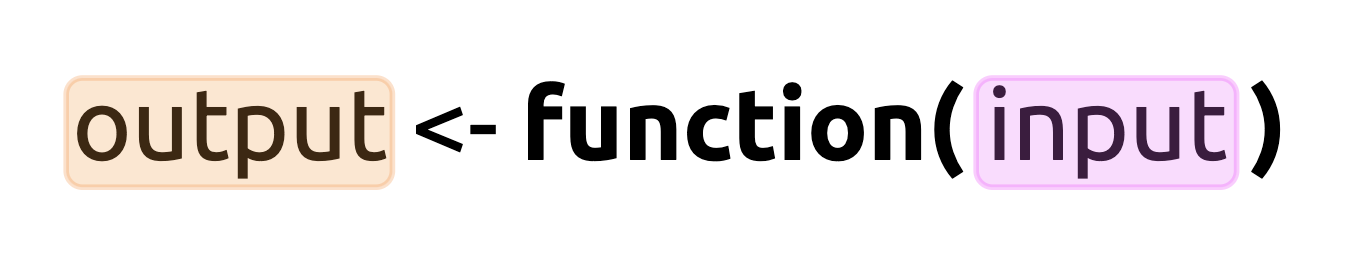
\includegraphics[width=19.06in]{img/pipe-args-01} \end{center}

Becomes this:

\begin{center}
\includegraphics[width=22.56in]{img/pipe-args-02} \end{center}

\hypertarget{pipelines}{%
\subsubsection{Pipelines}\label{pipelines}}

As you can imagine, writing code like this can get complicated if we
wanted to use multiple functions (as we typically do), Without the pipe,
we have to write these as nested functions (i.e.~\texttt{h(f(x))}).

\begin{center}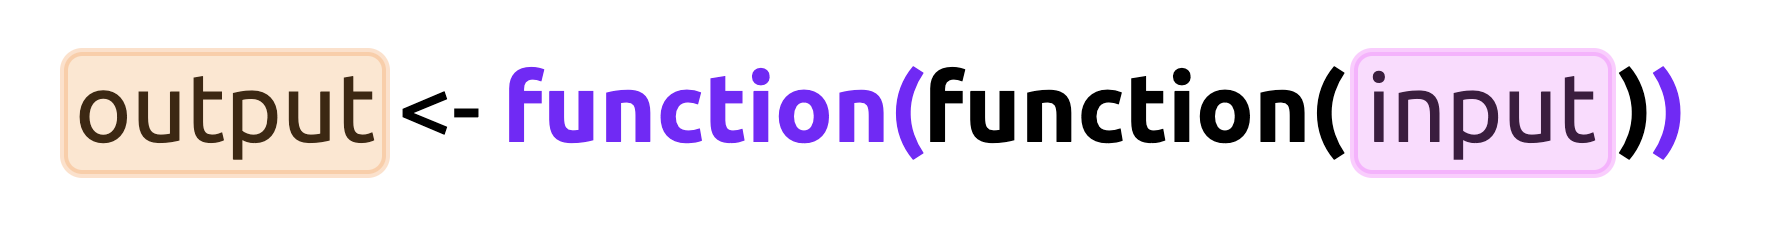
\includegraphics[width=24.81in]{img/pipe-args-03} \end{center}

With the pipe, we can rewrite this code to the following:

\begin{center}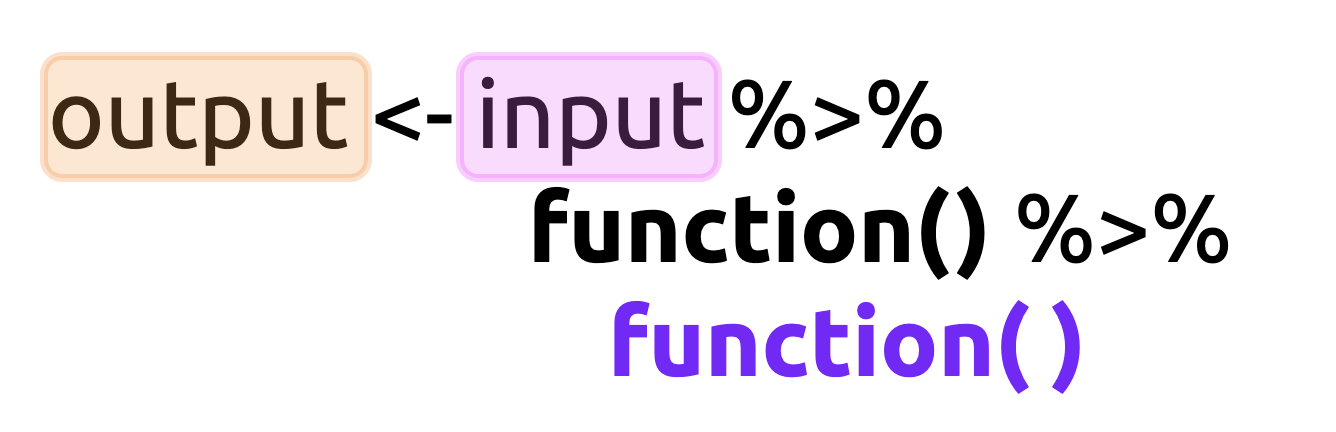
\includegraphics[width=18.56in]{img/pipe-args-04} \end{center}

Using the pipe makes code easier to 1) think about, 2) write, and 3)
read.

\hypertarget{exercise-6}{%
\subsubsection{exercise}\label{exercise-6}}

Pipe the \texttt{WikiCovid} to the \texttt{skimr::skim()} function:

\begin{Shaded}
\begin{Highlighting}[]
\NormalTok{WikiCovid }\SpecialCharTok{\%\textgreater{}\%} 
\end{Highlighting}
\end{Shaded}

\hypertarget{solution-6}{%
\subsubsection{solution}\label{solution-6}}

See the solution below:

\begin{Shaded}
\begin{Highlighting}[]
\NormalTok{WikiCovid }\SpecialCharTok{\%\textgreater{}\%}\NormalTok{ skimr}\SpecialCharTok{::}\FunctionTok{skim}\NormalTok{()}
\end{Highlighting}
\end{Shaded}

\begin{longtable}[]{@{}ll@{}}
\caption{Data summary}\tabularnewline
\toprule
& \\
\midrule
\endfirsthead
\toprule
& \\
\midrule
\endhead
Name & Piped data \\
Number of rows & 197 \\
Number of columns & 3 \\
\_\_\_\_\_\_\_\_\_\_\_\_\_\_\_\_\_\_\_\_\_\_\_ & \\
Column type frequency: & \\
character & 1 \\
numeric & 2 \\
\_\_\_\_\_\_\_\_\_\_\_\_\_\_\_\_\_\_\_\_\_\_\_\_ & \\
Group variables & None \\
\bottomrule
\end{longtable}

\textbf{Variable type: character}

\begin{longtable}[]{@{}lrrrrrrr@{}}
\toprule
skim\_variable & n\_missing & complete\_rate & min & max & empty &
n\_unique & whitespace \\
\midrule
\endhead
location & 0 & 1 & 2 & 32 & 0 & 197 & 0 \\
\bottomrule
\end{longtable}

\textbf{Variable type: numeric}

\begin{longtable}[]{@{}
  >{\raggedright\arraybackslash}p{(\columnwidth - 20\tabcolsep) * \real{0.13}}
  >{\raggedleft\arraybackslash}p{(\columnwidth - 20\tabcolsep) * \real{0.09}}
  >{\raggedleft\arraybackslash}p{(\columnwidth - 20\tabcolsep) * \real{0.13}}
  >{\raggedleft\arraybackslash}p{(\columnwidth - 20\tabcolsep) * \real{0.10}}
  >{\raggedleft\arraybackslash}p{(\columnwidth - 20\tabcolsep) * \real{0.11}}
  >{\raggedleft\arraybackslash}p{(\columnwidth - 20\tabcolsep) * \real{0.03}}
  >{\raggedleft\arraybackslash}p{(\columnwidth - 20\tabcolsep) * \real{0.07}}
  >{\raggedleft\arraybackslash}p{(\columnwidth - 20\tabcolsep) * \real{0.07}}
  >{\raggedleft\arraybackslash}p{(\columnwidth - 20\tabcolsep) * \real{0.10}}
  >{\raggedleft\arraybackslash}p{(\columnwidth - 20\tabcolsep) * \real{0.11}}
  >{\raggedright\arraybackslash}p{(\columnwidth - 20\tabcolsep) * \real{0.06}}@{}}
\toprule
skim\_variable & n\_missing & complete\_rate & mean & sd & p0 & p25 &
p50 & p75 & p100 & hist \\
\midrule
\endhead
n\_vaccinated & 0 & 1.00 & 8027773.08 & 48678725.27 & 22 & 32969.0 &
2.5e+05 & 1165669.00 & 595234872.0 & ▇▁▁▁▁ \\
perc\_of\_pop & 14 & 0.93 & 15.74 & 19.15 & 0 & 1.6 & 6.9e+00 & 24.85 &
111.3 & ▇▂▁▁▁ \\
\bottomrule
\end{longtable}

As we can see, \texttt{the\ skim()} output gives us a lot of descriptive
information about the variables (columns) in \texttt{WikiCovid}. A brief
summary of these statistics is provided below:

\textbf{Character variables} We can see none of the data in
\texttt{location} are missing (\texttt{n\_missing} and
\texttt{complete\_rate}). \texttt{Skimr::skim()} also shows us the
\texttt{min}, \texttt{max}, \texttt{empty}, \texttt{n\_unique}, and
\texttt{whitespace}.

\textbf{Numeric variables: Location statistics}\\
- the \texttt{mean} (or average) gives us the expected value for each
variable\\
- the median (as \texttt{p50}) or the `center' value for each variable.
Half of the values are above, and half are below.

\textbf{Numeric variables: Spread statistics}\\
- the lowest value for each variable, or minimum (as \texttt{p0})\\
- the highest value for each variable, or maximum (as \texttt{p100})\\
\emph{Together, these two values can give us the range, which is the
difference between the maximum and minimum values}

\textbf{\emph{Do you notice anything strange?}}

Now we are ready to start visualizing!

\begin{center}\rule{0.5\linewidth}{0.5pt}\end{center}

\end{document}
